% !TeX root = ../main.tex
% Add the above to each chapter to make compiling the PDF easier in some editors.

\chapter{System Design}\label{chapter:sys_design}
This chapter presents the system design in detail. It will start with an introduction of the main features of the framework used for developing the chatbot, Rasa, including its features and how it interacts with the Telegram Bot API that is used to communicate with the users. Then it will show how stress detection is done with adaptive sampling. After that, it will explain how eating behavior data is collected and processed. Furthermore, the conversation flow is going to be delivered in detail. The last section will present how data is persisted.

\section{The Rasa Framework}
Rasa (\citeyear{10_rasa}) is an open-source framework based on natural language processing (NLP) for developing chatbots. This section introduces why it is used and its main components and features.

\subsection{Why Rasa}
The most important reason for choosing Rasa was that the software developed in this thesis is based on the project of \citeauthor{17_ludwig} (\citeyear{17_ludwig}) who chose Rasa as the underlying framework. However, apart from that, there are certain benefits that Rasa comes with that serve very well the goals of this project. Firstly, Rasa is completely open-source, which means it is not only free to use but also easy to customize. For example, the chatbot was designed to collect user's location data for automatic timezone conversion and image data for food reflection, and this feature can be easily fulfilled by modifying the social network platform connector of Rasa, which will be shown in detail later this section. Secondly, Rasa comes along with a sophisticated natural language understanding (NLU) model for common English. Developers only need to provide a small set of sample data for it to predict user intents with a low error rate. Thirdly, unlike its commercial counterparts such as Amazon’s Lex and Google's Dialogflow, it does not depend on cloud infrastructure, and can instead be run as a piece of self-host software (\cite{24_why_rasa}). This makes it easy to integrate other components into the chatbot. For example, a separate scheduler which not only schedules messages but also does on-the-flight training of the data was developed alongside the chatbot and interacts well with the latter.

\subsection{Main Components of Rasa}
\citeauthor{16_martin} (\citeyear{17_ludwig}) gave a general review of the components of Rasa. This subsection is therefore based on his review and the requirements of this project.

\subsubsection{Rasa NLU}
As the name suggests, this is the NLU module of the Rasa framework which is responsible for understanding the user input. Specifically, this module helps identify the intent of the user and entities in the application domain from English sentences the user sends to the bot. This is done by training an NLU model based on sample data provided by the developer. In the context of this work, the usage of this module is mainly limited to identifying users' intend to describe food and report stress. For each user input, another module called Rasa Core utilizes the NLU model to calculate the probability of each pre-defined intent and predicts the intent with the highest probability.

\subsubsection{Rasa Core}
While Rasa NLU takes care of understanding what a user says, Rasa Core takes the initiative to respond to the user properly. Like Rasa NLU, Rasa Core uses machine learning to train its predictive model. The training data is a set of sample conversations in the markdown format. This training data is called Rasa stories.

\subsubsection{Rasa Stories}
The markdown file records all stories used as training data for Rasa Core. Every single story starts with "\#\#" followed by its name, and contains one or more user intent(s), denoted with "*", and one or more Rasa action(s), denoted by "-". Here is one example of a story:\bigskip

\begin{lstlisting}
## reflect food
* reflect_food
  - action_send_image
* describe_food
  - action_save_data
  - utter_more_or_less
\end{lstlisting}

\bigskip
\subsubsection{Rasa Actions}
An action is a response the chatbot performs to the user intent. There are two types of actions, namely \emph{utterances} and \emph{custom actions}. Utterances have to be defined in a markdown file following a certain format. Below is an example of an utterance which asks the user if he or she has eaten anything:\bigskip

\begin{lstlisting}
utter_did_you_eat:
- text: "Did you eat anything whilst you were stressed?"
  buttons:
  - title: Yes
    payload: /affirm
  - title: No
    payload: /deny
\end{lstlisting}

\bigskip
The uttered messages can have one or multiple types, which in the above case are a piece of text with two buttons. Each button can carry a payload which refers to a particular intent. When the user presses the button, its corresponding intent is sent back to the bot.

Unlike utterances that are relatively restricted, custom actions call a web server that can perform any task defined by the server and send any number of messages to the user. A typical way of implementing custom actions is to use the Python SDK offered by Rasa. \hyperref[ssec:custom_action]{Subsection~\ref*{ssec:custom_action}} looks into details of custom actions implemented in this project.

\subsubsection{Rasa Slots}
Slots are key-value stores that provide memory to the chatbot. It can be viewed as variables shared among different actions in the Rasa service, as well as a bridge between the metadata used for training and the code used for handle actions. More specifically, slots can be get and set via stories (\autoref{story_slot}) or by calling getter and setter functions in custom actions (\autoref{action_slot}). This is otherwise impossible as, without slots, actions would become stateless.\bigskip

\begin{lstlisting}[label={story_slot},caption={Using slots in stories to save user's stress level},captionpos=b]
* previous_stress
  - utter_ask_stress_level
* tell_stress_level{"level":"1"}
  - slot{"level":"1"}
  - action_save_data
  - utter_did_you_eat
* deny
  - utter_see_you
\end{lstlisting}

\bigskip
\begin{lstlisting}[label={action_slot},caption={Getting and setting slots in a custom action to relate entries in persistent data. "photo\_timestamps" and "reference\_ids" are used to find the correct photos to be send to the user in the future\, which help the user to reflect food.},language=Python,captionpos=b]
class ActionSaveData(Action):
    def name(self) -> Text:
        return "action_save_data"
    # some lines omitted
    def run(self,
            dispatcher: CollectingDispatcher,
            tracker: Tracker,
            domain: Dict[Text, Any]) -> List[Dict[Text, Any]]:
        # some lines omitted
        reference_ids = []
        photo_timestamps = []
        if (intent == "describe_food"):
            entity = "food"
            try:
                reference_ids = ';'.join(tracker.get_slot('reference_ids'))
                photo_timestamps = ';'.join(
                    tracker.get_slot('photo_timestamps'))
        # some lines omitted
        entry_id = self.addToProfile(
                tracker.latest_message['text'].replace(',', ';'),
                tracker.sender_id,
                intent,
                entityValue,
                photo_timestamps,
                reference_ids)
        return [SlotSet("photo_timestamps", []),
                SlotSet("reference_ids", [entry_id])]
\end{lstlisting}

\bigskip
While Rasa was selected as the underlying platform the chatbot is based on, Telegram was chosen as the social platform to run the chatbot on. This was a straightforward choice since \citeauthor{17_ludwig} was already using Telegram in his project (and it's worth reminding that the code of this project is based on the one of \citeauthor{17_ludwig}). And it turned out that it was easy to find enough Telegram users from a wide variety of timezones to participate in the user trial.

Rasa provided a Telegram connector which acts as an agent connecting to the Telegram Bot API. However, since Rasa is based on NLU, no photo or location data is handled by default. It is nevertheless necessary to deal with such information as part of the feature of this bot. The next subsection presents necessary changes made to this connector to facilitate these features.

\subsection{Interaction with the Telegram Bot API}
The built-in Telegram channels provided by Rasa consists of two classes, namely \emph{TelegramOutput} and \emph{TelegramInput}, controlling the handling of output and input messages to users, respectively. By default, the \emph{TelegramInput} channel only handles text data. In order for the handling of images and locations to work, this class was modified and renamed to \emph{TelegramPlusInput}. Additionally, some other functionalities are added, which are explained below.

\subsubsection{User Registration}
A new user needs to be registered before his or her data can be recorded. Details of the registration process will be presented in \autoref{ssec:onboarding}. As a standard approach, this registration is done right after the user issues the \emph{/start} command to the bot. It creates a folder and two CSV files to record the user data, without which the chatbot continues to interact with the user, but no data is collected. In case there was an error in the standard registration process (e.g. the user issued the \emph{/start} command when the server is down), the \emph{TelegramPlusInput} channel triggers a backup process in case that a user message is received, but no folder of the respective user is found.

\subsubsection{User Location and Timezone}
The bot needs to collect the timezone data from the users to schedule messages to them at the right time. The timezones are calculated based on locations sent by the users. On Telegram, a location is a JSON object consisting of the latitude and longitude. The \emph{TelegramPlusInput} connector captures this object and converts it into a Python string that can be recognized by Rasa NLU. The format of this string is defined as follows:

\begin{lstlisting}
## intent:tell_lat_lng
- "lng":0.0, "lat":0.0
- "lat":0.0, "lng":0.0
\end{lstlisting}

\bigskip
and the respective logic in the Telegram connector is

\begin{lstlisting}[language=Python]
elif self._is_location(msg):
    text = '{{"lng":{0}, "lat":{1}}}'.format(
        msg.location.longitude, msg.location.latitude
    )
    # store timezone information of the user
    tf = TimezoneFinder()
    latitude, longitude = msg.location.latitude, msg.location.longitude
    timezone_str = tf.timezone_at(
        lng=longitude, lat=latitude)
    with open('./user_data/timezones.csv', 'a', newline='') as csvfile:
        writer = csv.writer(
            csvfile,
            delimiter=',',
            quotechar='|',
            quoting=csv.QUOTE_MINIMAL)
        writer.writerow(
            [datetime.now(), str(msg.chat.id), timezone_str])
\end{lstlisting}

\subsubsection{Photos}
Another important feature is to process photos sent by users to the bot. If the bot detects a user being stressed and eating at the same time, instead of asking the user to describe immediately in text what he or she is eating, it asks the user to take a photo of the food. This design choice was made under the assumption that it is relatively easier for someone who is eating to take and send a photo than to text description of the food. In addition, the photos collected were included in the survey which collects users' opinions on comfort food at the end of the user study. When a user sends a file (e.g. a photo) in a Telegram conversation, Telegram saves the photo on its server that can be accessed via the \emph{chat\_id} which identifies the chat and a unique \emph{file\_id} by calling the Telegram Bot API. With this feature, the Rasa bot does not need to save the photos locally, but only need to save the \emph{chat\_id} and \emph{file\_id}. This feature is implemented by the following code in the \emph{TelegramPlusInput} connector. \bigskip

\begin{lstlisting}[language=Python]
if not hasattr(msg, 'photo'):
    return response.text("success")
if len(msg.photo) == 0:
    print("Not a photo")
    return response.text("success")
max_size = 0
for photo in msg.photo:
    if photo.file_size > max_size:
        max_size = photo.file_size
        file_id = photo.file_id
reference_id = ''
try:
    with open(
      './user_data/' + str(str(msg.chat.id)) + '/profiles.csv',
        newline='') as csvfile:
        reader = csv.reader(
            csvfile, delimiter=',', quotechar='|')
        for row in reader:
            reference_id = row[0]
except FileNotFoundError:
    pass
with open(
  './user_data/' + str(str(msg.chat.id)) + '/photos.csv',
  'a',
  newline='') as csvfile:
    writer = csv.writer(
        csvfile, delimiter=',', quotechar='|', quoting=csv.QUOTE_MINIMAL)
    writer.writerow([datetime.now(), str(
        msg.chat.id), file_id, reference_id])
return response.text("success")
\end{lstlisting}

\subsubsection{Naming of the Chatbot}
The history of chatbot is closely coupled with that of artificial intelligence, with the goal of mimicking humans and the challenge of passing the Turing's test (\cite{38_turing}). Since it's earliest days, chatbot has been given human-like names, from ELIZA to PARRY (\cite{37_early_chatbots_1}). In fact, these names came about to sound like humans much earlier than chatbots themselves start to get out of the rule-based zone and use more intelligent means (such as machine learning) to communicate with humans (\cite{36_early_chatbots}). Apart from this tradition, is it widely researched that having human-like names could help a chatbot to be perceived more human by the actual human chatting with it (\cite{35_chatbot_name_1, 34_chatbot_name}). Therefore, it is crucial to name the chatbot. The bot in this project was named Demezys, which is a combination of \emph{Demeter} and \emph{Oizys}. Demeter is the Greek goddess of agriculture (\cite{39_demeter}) and Oizys the goddess of misery, anxiety, grief, and depression (\cite{40_oizys}). This name symbolizes the combination of eating and stress at a spiritual level.

\subsection{Training Data}
This subsection explains the training data used to train Rasa Core and Rasa NLU.

\subsubsection{domain.yml}
The declaration of actions, intents, slots and templates to each utterance are saved in \emph{domain.yml} (see \autoref{domain}).

\subsubsection{NLU}
All training data regarding the intents is saved in \emph{nlu.md} (see \autoref{nlu}). It includes the food data that is used to predict the \emph{describe\_food} intent. The items are determined according to the training data from \citeauthor{17_ludwig}. In addition, phrases such as "I didn't eat anything when I was stressful" and "Nothing" was added to address the case when a user has no food to report.

\subsubsection{Stories}
The stories are defined in \emph{stories.md} (see \autoref{stories}). Details about the conversation flow is to be discussed in \autoref{flow}.

\subsection{Custom Actions} \label{ssec:custom_action}
Some of the important features of Demezys was implemented in the custom actions. This subsection discusses the details of them. A full list of custom actions can be found at \autoref{domain}.

\subsubsection{User Registration}
The user registration is done via the \emph{action\_register\_user} action. This action is triggered when the user issues the \emph{/start} command to Demezys. The file path \emph{./user\_data} is created, followed by the creation of the file \emph{./user\_data/users.csv}, which saves the \emph{chat\_id} of the user. Afterwards, it creates a path \emph{./user\_data/<chat\_id>} for holding the user data, and two files \emph{profiles.csv} and \emph{photos.csv} under that path.\bigskip

\begin{figure}
  \begin{forest}
    for tree={
      font=\ttfamily,
      grow'=0,
      child anchor=west,
      parent anchor=south,
      anchor=west,
      calign=first,
      edge path={
        \noexpand\path [draw, \forestoption{edge}]
        (!u.south west) +(7.5pt,0) |- node[fill,inner sep=1.25pt] {} (.child anchor)\forestoption{edge label};
      },
      before typesetting nodes={
        if n=1
          {insert before={[,phantom]}}
          {}
      },
      fit=band,
      before computing xy={l=15pt},
    }
  [.
    [user\_data
      [timezones.csv]
      [users.csv]
      [user\_1
        [photos.csv]
        [profiles.csv]
      ]
      [user\_2
        [photos.csv]
        [profiles.csv]
      ]
      [... more users]
    ]
  ]
  \end{forest}
  \caption{Structure of data persistence}
  \label{fig:file_treev}
\end{figure}

\subsubsection{Saving Data}
\emph{action\_save\_data} is responsible for saving the stress and eating data in the \emph{profiles.csv} files. The format of the data is illustrated in \autoref{data_persis}. It first checks the latest intent of the user in order to take the corresponding actions.

If the intent was \emph{describe\_food}, it will try to get the slot values of \emph{reference\_ids} and \emph{photo\_timestamps}, which potentially link the food photo(s) being described to a previous stress entry, building the connection between stress and eating. It could be, however, that the user was not describing food according to photo(s). This situation can be broken down into two cases. One is that the user is describing food right after he or she told the bot the stress level. In this case, the \emph{describe\_food} entry is linked to the latest stress entry. The other case is that the user is describing food at the end of the day which does not refer to a specific stress entry but the day in general. In such a case, no stress entry is linked to the \emph{describe\_food} entry.

If the intent was not \emph{describe\_food}, it will directly extract the entity and save the data entry together with the intent.

\subsubsection{Sending Image/Imanges}
\emph{action\_send\_image} extracts all the \emph{file\_id}s of the photos a user has sent to Demezys during the day and sends the photos back to the user by calling the Telegram Bot API, together with a text prompting the user to reflect food according to the photos. If no photos are found, it asks the user to reflect food directly. If the user was not detected stressed during the day, it directly sends the \emph{utter\_pieces} action to the user, which asks about how many pieces of meal/snacks the user has had during the day, bypassing the process of describing food.

\subsubsection{Asking Location}
After a user is registered, Demezys asks the user to send his or her location via Telegram. This is done by \emph{action\_ask\_location}. It prompts the user with a text saying "Please send your location to me. I need this information to schedule message to you in the right time. Please use the Telegram built-in function to send location, and \textbf{DO NOT} send a text message." while sending a photo (\autoref{fig:share-loc}) instructing the user to do so, in case some people are not familiar with the share-location feature of Telegram.

\begin{figure}[ht]
  \centering
  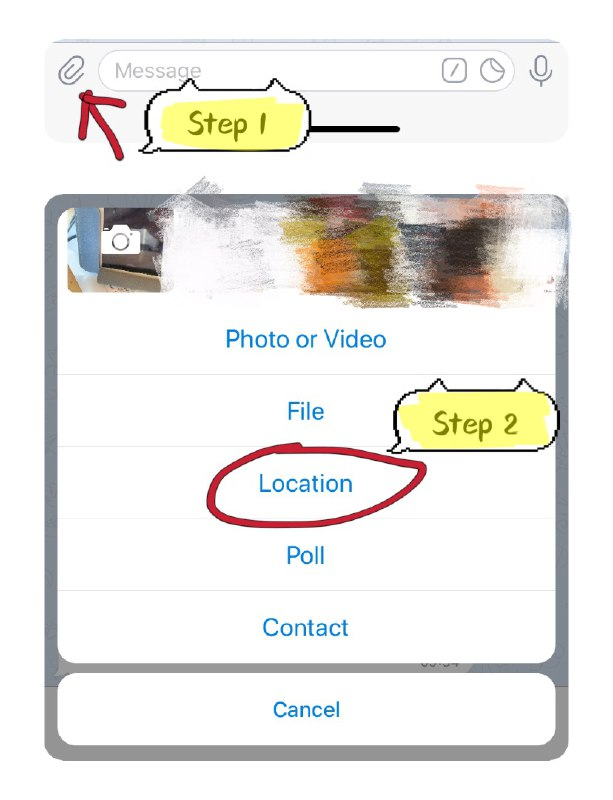
\includegraphics[width=0.5\textwidth]{fig-share-loc}
  \caption{Instruction to sharing location via Telegram}
  \label{fig:share-loc}
\end{figure}

\section{Stress Detection with Adaptive Sampling}
As discussed in \autoref{scope_stress_detection}, collecting stress data relies solely on adaptive sampling. This section provides details on how the sampling works.

In this project, stress is measured with levels from 0 to 5, 0 being not stressed and 5 being extremely stressed. This straightforward one-dimension scaling has proven to be effective in measuring stress and is being widely used in psychology questionnaires (\cite{41_stress_scale}). In addition, users only need to spend a minimal amount of time to answer such a question, making the chatbot less intrusive.

The stress samplings are done by a scheduler written in Python. It schedules messages on a per-user basis. Upon registration, a user sends his or her location to Demezys, and the location is converted to its corresponding timezone and saved in the \emph{timezones.csv} file together with the \emph{chat\_id}. Initially, the scheduler sends four messages per day, three of which being \emph{detect\_stress} and one being \emph{reflect\_food}. \emph{detect\_stress} triggers the bot to ask "are you feeling stressed", entering into the process of collecting the user's stress level. \emph{reflect\_food} asks the user to reflect on the food he or she has eaten when feeling stressed during the day, as well as the amount of food. The scheduling of \emph{reflect\_food} is set to be 21:00 every day, with the assumption that this is the time between dinner and sleep for most of the people. \emph{detect\_stress} are initially scheduled 3 times per day, at 9:00, 13:00, and 19:00, which are slightly later than the times when most people are likely to have meals. The bot is designed to ask about the stress level of one hour before, in case the user says he or she is not stressed at the moment (\autoref{flow}). The scheduling scheme is therefore assumed to hit the time when the users are eating with a higher possibility than random scheduling.

To better understand when participants are likely to feel stressed on an individual basis, an adaptive scheduling model was developed. This model not only adapts the scheduled timestamps based on historical values but also the number of stress samplings per day. This reduces the number of times when the chatbot asks about stress for those who feel stressed less frequently than others (\autoref{fig:adapt-stress}), ensuring that Demezys is not "spamming" its users.

The adaptive sampling is achieved by using k-means clustering on previous timestamps of stress entries. First, all previous stress entries are collected, with the corresponding timestamps and stress levels. All timestamps were collected in the 'Europe/Berlin' timezone. Then, the timestamps are converted to the local time of the users according to the timezone saved in \emph{timezones.csv} Afterwards, the difference between each timestamp and the timestamp of the start of its day is calculated and saved. For example, for timestamp \texttt{2020-04-07 13:00:50} is transformed to 46850 seconds, which is the difference between itself and the start of the day (\texttt{2020-04-07 00:00:00}). Each saved time difference is a data point in integer form. Finally, each data point is copied \emph{n-1} times where \emph{n} is the stress level corresponding to that data point. This is to make sure that timestamps associated with higher levels of stress get more weight in the clustering training so that the training result can better predict the time when the user is likely to feel more stressed. This is based on the intuitive assumption that immense stress does not come and go abruptly so that a person is likely to feel some level of stress shortly before and after the timestamp when he or she is feeling a high level of stress.

The centroid of each cluster is converted back to a timestamp from its integer form. The \texttt{hour}s of the centroids will be the hours when Demezys schedules the new \emph{detect\_stress} message the coming day. The k-means clustering algorithm is applied to all 18 participants whose \emph{chat\_id}s are even numbers, among the total of 33 participants. Participants with odd \emph{chat\_id}s receive reminders at fixed times per day, 3 times a day as the controlled group. The participants are not informed of this setting.

\section{Collection and Processing of Eating Behavior Data}
There are three types of eating behavior data collected, namely food descriptions, amount compared to the non-stress state, and the number of pieces.

\subsection{Food Descriptions}
Food descriptions are collected whenever a user tells Demezys that he or she was stressed one hour ago and was eating then. In addition, if there is at least one record with a positive stress level during the day, the user will be prompted to give food descriptions either according to the photo(s) he or she has sent during the day, or plainly if there is no photo. To collect food descriptions, Demezys asks the user either of the following questions

\begin{itemize}
  \item Hi, time to reflect what you've eaten when you were stressed. Please describe the food on the photo(s).
  \item Please describe the food you've eaten when you felt stressed today.
\end{itemize}

according to the situation. Users' answers to these questions are saved into \emph{profiles.csv} as food descriptions.

Towards the end of this study, the food items from the descriptions were extracted manually and sent back to the users for comfort-food labeling. The binary label is added back to each food record for training the prediction model.

\subsection{Food Amount Compared to the Non-Stress State}
Right after food descriptions, the food amount compared to the non-stress state is asked at the end of each day in case the user has reported as least once a possitive stress level. This is done by the following action

\begin{lstlisting}
utter_more_or_less:
- text: "Was it more or less than the amount you would normally eat when you're *not* stressed?"
  buttons:
  - title: More
    payload: /tell_more_or_less{"more_or_less":"more"}
  - title: Less
    payload: /tell_more_or_less{"more_or_less":"less"}
  - title: Same
    payload: /tell_more_or_less{"more_or_less":"same"}
\end{lstlisting}

where three buttons are presented to the user. The value of the slot \emph{more\_or\_less} is recorded. 

\section{Conversation Flow} \label{flow}

\subsection{Onboarding} \label{ssec:onboarding}


\section{Data Persistence} \label{data_persis}
